%% CG vs steepest descent on the 100x100 grid Laplacian (generated by figs_c5ch02.py).
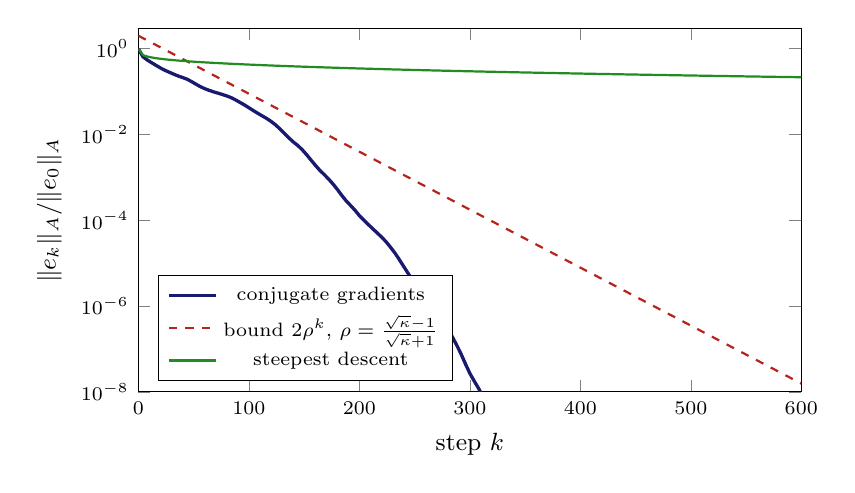
\begin{tikzpicture}
\begin{axis}[width=10cm,height=6.2cm,ymode=log,xmin=0,xmax=600,ymin=1e-8,ymax=3,xlabel={step $k$},ylabel={$\|e_k\|_A/\|e_0\|_A$},
  tick label style={font=\scriptsize},label style={font=\small},legend style={font=\scriptsize,at={(0.03,0.03)},anchor=south west},
  ytick={1e-8,1e-6,1e-4,1e-2,1}]
\addplot[MidnightBlue,very thick] coordinates {(0,1.000e+00) (4,6.533e-01) (8,5.451e-01) (12,4.700e-01) (16,4.082e-01) (20,3.544e-01) (24,3.134e-01) (28,2.823e-01) (32,2.543e-01) (36,2.310e-01) (40,2.128e-01) (44,1.947e-01) (48,1.716e-01) (52,1.493e-01) (56,1.306e-01) (60,1.170e-01) (64,1.069e-01) (68,9.858e-02) (72,9.194e-02) (76,8.567e-02) (80,7.918e-02) (84,7.207e-02) (88,6.382e-02) (92,5.581e-02) (96,4.876e-02) (100,4.201e-02) (104,3.609e-02) (108,3.122e-02) (112,2.720e-02) (116,2.371e-02) (120,2.023e-02) (124,1.689e-02) (128,1.354e-02) (132,1.074e-02) (136,8.415e-03) (140,6.758e-03) (144,5.607e-03) (148,4.479e-03) (152,3.436e-03) (156,2.572e-03) (160,1.938e-03) (164,1.478e-03) (168,1.176e-03) (172,9.213e-04) (176,7.074e-04) (180,5.261e-04) (184,3.824e-04) (188,2.842e-04) (192,2.218e-04) (196,1.715e-04) (200,1.284e-04) (204,1.010e-04) (208,8.007e-05) (212,6.381e-05) (216,5.109e-05) (220,4.087e-05) (224,3.191e-05) (228,2.383e-05) (232,1.752e-05) (236,1.229e-05) (240,8.468e-06) (244,5.844e-06) (248,4.025e-06) (252,2.781e-06) (256,1.892e-06) (260,1.347e-06) (264,9.680e-07) (268,6.927e-07) (272,5.098e-07) (276,3.724e-07) (280,2.753e-07) (284,1.941e-07) (288,1.243e-07) (292,7.685e-08) (296,4.491e-08) (300,2.692e-08) (304,1.777e-08) (308,1.194e-08) (312,7.529e-09) (316,5.074e-09) (320,3.635e-09) (324,2.511e-09) (328,1.659e-09) (332,1.009e-09) (336,1.000e-09) (340,1.000e-09) (344,1.000e-09) (348,1.000e-09) (352,1.000e-09) (356,1.000e-09) (360,1.000e-09) (364,1.000e-09) (368,1.000e-09) (372,1.000e-09) (376,1.000e-09) (380,1.000e-09) (384,1.000e-09) (388,1.000e-09) (392,1.000e-09) (396,1.000e-09) (400,1.000e-09) (404,1.000e-09) (408,1.000e-09) (412,1.000e-09) (416,1.000e-09) (420,1.000e-09) (424,1.000e-09) (428,1.000e-09) (432,1.000e-09) (436,1.000e-09) (440,1.000e-09) (444,1.000e-09) (448,1.000e-09) (452,1.000e-09) (456,1.000e-09) (460,1.000e-09) (464,1.000e-09) (468,1.000e-09) (472,1.000e-09) (476,1.000e-09) (480,1.000e-09) (484,1.000e-09) (488,1.000e-09) (492,1.000e-09) (496,1.000e-09) (500,1.000e-09) (504,1.000e-09) (508,1.000e-09) (512,1.000e-09) (516,1.000e-09) (520,1.000e-09) (524,1.000e-09) (528,1.000e-09) (532,1.000e-09) (536,1.000e-09) (540,1.000e-09) (544,1.000e-09) (548,1.000e-09) (552,1.000e-09) (556,1.000e-09) (560,1.000e-09) (564,1.000e-09) (568,1.000e-09) (572,1.000e-09) (576,1.000e-09) (580,1.000e-09) (584,1.000e-09) (588,1.000e-09) (592,1.000e-09) (596,1.000e-09) (600,1.000e-09)};
\addlegendentry{conjugate gradients}
\addplot[BrickRed,dashed,thick,domain=0:600,samples=3] {2*0.969369^x};
\addlegendentry{bound $2\rho^k$, $\rho=\frac{\sqrt\kappa-1}{\sqrt\kappa+1}$}
\addplot[ForestGreen,thick] coordinates {(0,1.000e+00) (4,7.107e-01) (8,6.570e-01) (12,6.243e-01) (16,6.004e-01) (20,5.814e-01) (24,5.655e-01) (28,5.519e-01) (32,5.399e-01) (36,5.291e-01) (40,5.192e-01) (44,5.102e-01) (48,5.019e-01) (52,4.941e-01) (56,4.868e-01) (60,4.799e-01) (64,4.734e-01) (68,4.672e-01) (72,4.613e-01) (76,4.557e-01) (80,4.503e-01) (84,4.451e-01) (88,4.401e-01) (92,4.353e-01) (96,4.307e-01) (100,4.262e-01) (104,4.219e-01) (108,4.177e-01) (112,4.136e-01) (116,4.096e-01) (120,4.058e-01) (124,4.021e-01) (128,3.984e-01) (132,3.949e-01) (136,3.915e-01) (140,3.881e-01) (144,3.848e-01) (148,3.816e-01) (152,3.785e-01) (156,3.755e-01) (160,3.725e-01) (164,3.696e-01) (168,3.668e-01) (172,3.640e-01) (176,3.612e-01) (180,3.586e-01) (184,3.560e-01) (188,3.534e-01) (192,3.509e-01) (196,3.484e-01) (200,3.460e-01) (204,3.436e-01) (208,3.413e-01) (212,3.390e-01) (216,3.368e-01) (220,3.346e-01) (224,3.324e-01) (228,3.303e-01) (232,3.282e-01) (236,3.261e-01) (240,3.241e-01) (244,3.221e-01) (248,3.202e-01) (252,3.183e-01) (256,3.164e-01) (260,3.145e-01) (264,3.127e-01) (268,3.109e-01) (272,3.091e-01) (276,3.073e-01) (280,3.056e-01) (284,3.039e-01) (288,3.022e-01) (292,3.006e-01) (296,2.990e-01) (300,2.974e-01) (304,2.958e-01) (308,2.942e-01) (312,2.927e-01) (316,2.911e-01) (320,2.896e-01) (324,2.882e-01) (328,2.867e-01) (332,2.853e-01) (336,2.838e-01) (340,2.824e-01) (344,2.810e-01) (348,2.797e-01) (352,2.783e-01) (356,2.770e-01) (360,2.756e-01) (364,2.743e-01) (368,2.730e-01) (372,2.718e-01) (376,2.705e-01) (380,2.693e-01) (384,2.680e-01) (388,2.668e-01) (392,2.656e-01) (396,2.644e-01) (400,2.632e-01) (404,2.620e-01) (408,2.609e-01) (412,2.597e-01) (416,2.586e-01) (420,2.575e-01) (424,2.564e-01) (428,2.553e-01) (432,2.542e-01) (436,2.531e-01) (440,2.520e-01) (444,2.510e-01) (448,2.499e-01) (452,2.489e-01) (456,2.478e-01) (460,2.468e-01) (464,2.458e-01) (468,2.448e-01) (472,2.438e-01) (476,2.428e-01) (480,2.419e-01) (484,2.409e-01) (488,2.399e-01) (492,2.390e-01) (496,2.380e-01) (500,2.371e-01) (504,2.362e-01) (508,2.353e-01) (512,2.344e-01) (516,2.335e-01) (520,2.326e-01) (524,2.317e-01) (528,2.308e-01) (532,2.299e-01) (536,2.290e-01) (540,2.282e-01) (544,2.273e-01) (548,2.265e-01) (552,2.256e-01) (556,2.248e-01) (560,2.240e-01) (564,2.232e-01) (568,2.223e-01) (572,2.215e-01) (576,2.207e-01) (580,2.199e-01) (584,2.191e-01) (588,2.183e-01) (592,2.176e-01) (596,2.168e-01) (600,2.160e-01)};
\addlegendentry{steepest descent}
\end{axis}
\end{tikzpicture}
